\chapter{Simulation de la Flotte IoT}

\section{Présentation du dataset}

\subsection{Source des données}

Le dataset utilisé est le \textbf{IoT Communication Security Dataset}, composé de 76\,000 entrées représentant des échanges MQTT typiques d'un écosystème IoT industriel. Chaque entrée décrit les caractéristiques d'une communication : protocole, longueur du payload, durée, type d'attaque éventuel, etc.

\subsection{Distribution des classes}

\begin{table}[H]
\centering
\caption{Distribution des classes dans le dataset}
\label{tab:dataset_classes}
\begin{tabular}{lrl}
\toprule
\textbf{Classe} & \textbf{Occurrences} & \textbf{Description} \\
\midrule
Normal & 43\,200 & Trafic IoT légitime \\
DoS & 12\,600 & Inondation de connexions/messages \\
MiTM & 8\,400 & Interception et modification de paquets \\
Replay & 5\,600 & Rejeu de messages capturés \\
FalsifiedData & 3\,900 & Injection de données falsifiées \\
Scanning & 1\,400 & Scan de ports et d'infrastructure \\
Malware & 840 & Comportements de type botnet \\
\bottomrule
\end{tabular}
\end{table}

\begin{figure}[H]
  \centering
  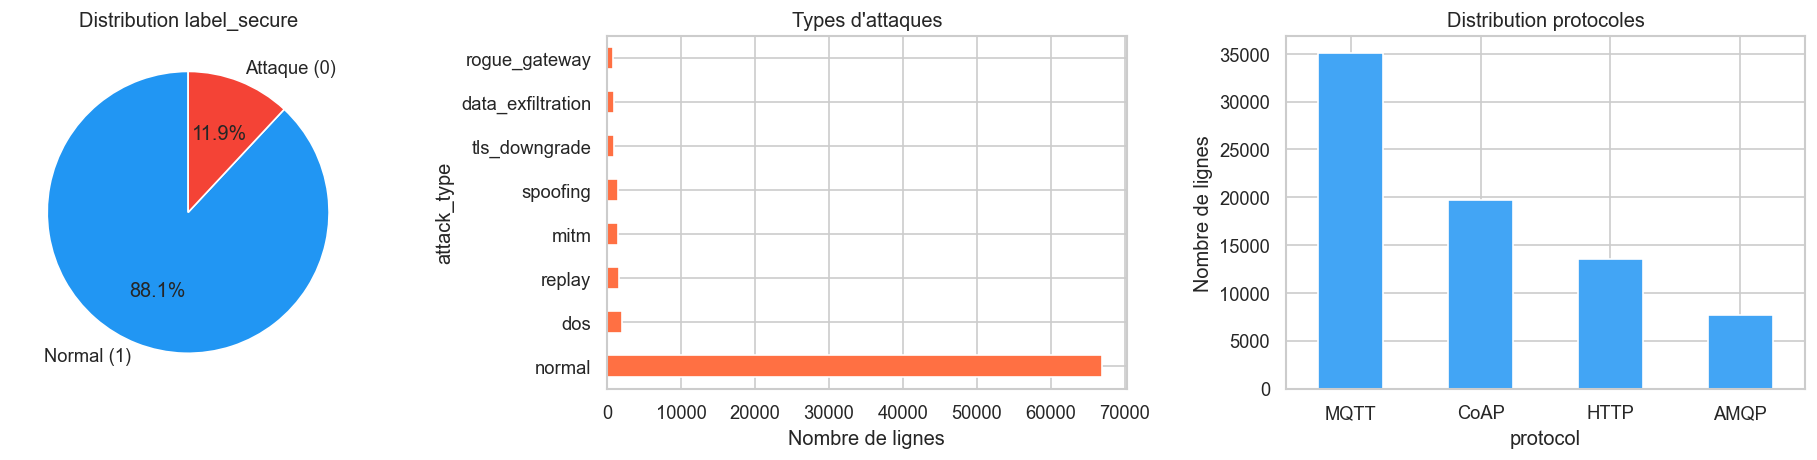
\includegraphics[width=0.7\textwidth]{figures/eda_classes_distribution.png}
  \caption{Distribution des classes dans le dataset IoT}
  \label{fig:class_dist}
\end{figure}

\section{Architecture du simulateur de flotte}

\subsection{Conception}

Le simulateur (\texttt{fleet\_sim.py}) est un programme Python multi-thread simulant une flotte de \textbf{50 dispositifs IoT} concurrents. Chaque dispositif :
\begin{itemize}
  \item Dispose d'un identifiant unique (\texttt{device-001} à \texttt{device-050}).
  \item Possède un certificat X.509 individuel émis par Vault.
  \item Publie des messages MQTT sur des topics dédiés (\texttt{iot/sensors/device-XXX/}).
  \item Reproduit fidèlement un sous-ensemble du dataset CSV (stratified sampling par classe).
\end{itemize}

\subsection{Structure du simulateur}

\begin{lstlisting}[language=python, caption=Extrait de fleet\_sim.py — classe DeviceSimulator]
class DeviceSimulator:
    def __init__(self, device_id: str, broker_config: dict,
                 cert_path: str, events: pd.DataFrame):
        self.device_id = device_id
        self.broker = broker_config
        self.cert = cert_path
        self.events = events
        self.client = mqtt.Client(
            client_id=device_id,
            protocol=mqtt.MQTTv5
        )
        self._configure_tls()

    def _configure_tls(self):
        """Configure mTLS avec les certificats Vault."""
        self.client.tls_set(
            ca_certs=f"{self.cert}/ca-chain.crt",
            certfile=f"{self.cert}/{self.device_id}.crt",
            keyfile=f"{self.cert}/{self.device_id}.key",
            tls_version=ssl.PROTOCOL_TLS_CLIENT
        )
        self.client.tls_insecure_set(False)

    def run(self):
        """Rejoue les événements du dataset."""
        self.client.connect(
            self.broker['host'],
            self.broker['port'],
            keepalive=60
        )
        self.client.loop_start()
        for _, event in self.events.iterrows():
            payload = self._format_payload(event)
            topic = f"iot/sensors/{self.device_id}/{event['type']}"
            self.client.publish(
                topic, json.dumps(payload), qos=1
            )
            # Respect du timing original du dataset
            time.sleep(event.get('interval', 0.1))
        self.client.loop_stop()
\end{lstlisting}

\subsection{Paramètres de simulation}

\begin{table}[H]
\centering
\caption{Paramètres de la simulation}
\label{tab:sim_params}
\begin{tabular}{ll}
\toprule
\textbf{Paramètre} & \textbf{Valeur} \\
\midrule
Nombre de dispositifs & 50 \\
Durée totale de simulation & $\sim$30 minutes \\
Messages/dispositif/minute & $\sim$50 \\
Total messages publiés & 76\,000 \\
Threads concurrents & 50 \\
QoS MQTT & 1 \\
\bottomrule
\end{tabular}
\end{table}

\section{Injection des patterns d'attaque}

Les patterns d'attaque sont rejoués tel quels depuis le dataset, préservant leur temporalité et leurs caractéristiques statistiques. Pour le scenario DoS, le flux de messages est intensifié pour reproduire l'inondation :

\begin{lstlisting}[language=python, caption=Injection du pattern DoS dans le simulateur]
def _inject_dos_pattern(self, base_rate: float) -> float:
    """Multiplie le taux de publication pour simuler une attaque DoS."""
    dos_multiplier = 10  # 10x le taux normal
    return base_rate / dos_multiplier  # intervalle réduit
\end{lstlisting}

\section{Résultats de la simulation}

La simulation a généré avec succès l'ensemble des 76\,000 événements. La capture réseau réalisée par Suricata a confirmé la cohérence du trafic avec le dataset source.

\begin{tcolorbox}[colback=green!5, colframe=green!50!black, title=Résultats de la simulation]
\begin{itemize}
  \item \textbf{76\,000 messages} publiés avec succès en mTLS.
  \item Taux de perte MQTT : \textbf{0\%} (QoS 1 avec retransmission).
  \item Les 50 dispositifs ont maintenu leurs connexions TLS simultanément.
  \item Fichier de capture : \texttt{results/analysis/step6/mqtt\_tls.pcap} (127 MB).
\end{itemize}
\end{tcolorbox}
